\begin{frame}
    \begin{itemize}
        \item Subtractive cutting/engraving by concentrated radiation
        \item Ablation: material removal by heating up
        \item Absorption of energy in the material
        \item Continuous or pulsed laser beams
        \item Almost all materials can be processed
    \end{itemize}
    \begin{figure}
        % https://commons.wikimedia.org/wiki/File:Bystronic_Laserschneiden.jpg
        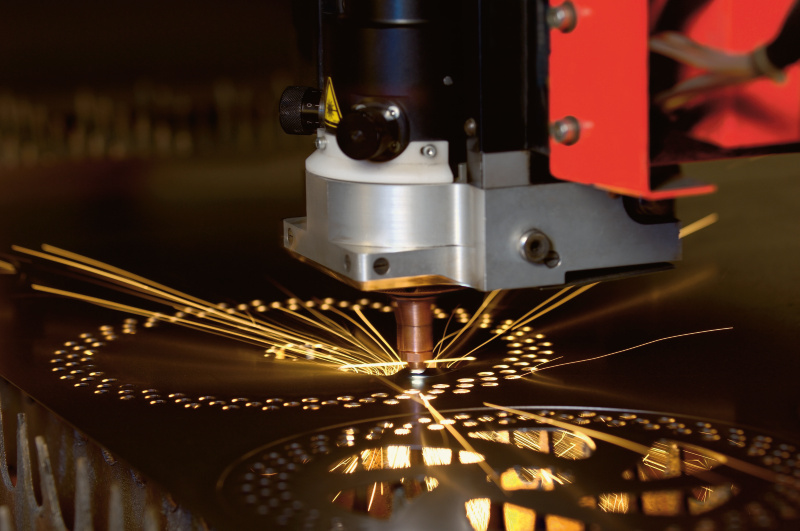
\includegraphics[height=4.5cm]{rapid-prototyping/bystronic-lasercutting.jpg}
        \caption{Bystronic: Laser Cutting}
    \end{figure}
\end{frame}